\section{Introducing differentiable binary arithmetic operations}
\label{sec:Nalu}
We define our problem as learning a set of static arithmetic operations between selected elements of a vector. E.g. for a vector $\mathbf{x}$ learn the function ${(x_5 + x_1) \cdot x_7}$. The approach taking in this paper, is to develop layers around specific operations, and then let each layer decide which inputs to include using backpropergation.

We develop these layers by analysing the theoretical issues in the Neural Arithmetic Logic Unit (NALU) \cite{trask-nalu}.

\subsection{Introducing NALU}
The Neural Arithmetic Logic Unit (NALU) consists of two sub-units; the $\text{NAC}_{+}$ and $\text{NAC}_{\bullet}$ that exclusively represent either the $\{+, -\}$ or the $\{\times, \div \}$ operations. The NALU then assumes that either $\text{NAC}_{+}$ or $\text{NAC}_{\bullet}$ will be selected exclusively, using a sigmoid gating-mechanism.

The $\text{NAC}_{+}$ and $\text{NAC}_{\bullet}$ are defined accordingly,
\begin{align}
W_{h_\ell, h_{\ell-1}} &= \tanh(\hat{W}_{h_\ell, h_{\ell-1}}) \sigma(\hat{M}_{h_\ell, h_{\ell-1}}) \label{eq:weight}\\
\textrm{NAC}_+:\ z_{h_\ell} &= \sum_{h_{\ell-1}=1}^{H_{\ell-1}} W_{h_{\ell}, h_{\ell-1}} z_{h_{\ell-1}} \label{eq:naca}\\
\textrm{NAC}_\bullet:\ z_{h_\ell} &= \exp\left(\sum_{h_{\ell-1}=1}^{H_{\ell-1}} W_{h_{\ell}, h_{\ell-1}} \label{eq:nacm}\log(|z_{h_{\ell-1}}| + \epsilon) \right)
\end{align}
where $\hat{\mathbf{W}}, \hat{\mathbf{M}} \in \mathbb{R}^{H_{\ell} \times H_{\ell-1}}$ are weight matrices and $z_{h_{\ell-1}}$ is the input. The matrices are combined using a tanh-sigmoid transformation to bias the parameters towards a $\{-1,0,1\}$ solution. Having $\{-1,0,1\}$ allows $\text{NAC}_{+}$ to be perform exact $\{+, -\}$ operations between elements of a vector.
The $\text{NAC}_{\bullet}$ uses an exponential-log transformation to create the $\{\times, \div \}$ operations (within $\epsilon$ precision).

The NALU combines these units with a gating mechanism $\mathbf{z} = \mathbf{g} \odot \text{NAC}_{+} + (1 - \mathbf{g}) \odot \text{NAC}_{\bullet}$ given $\mathbf{g} = \sigma(\mathbf{G} \mathbf{x})$. Thus allowing NALU to decide between all of $\{+, -, \times, \div\}$ using backpropagation.

\subsection{Challenges of gating between $\text{NAC}_{+}$ and $\text{NAC}_{\bullet}$}
\label{sec:methods:gatting-issue}
The sigmoid gating-mechanism in NALU, is problemtic in theory. Its purpose to select either $\text{NAC}_{+}$ or $\text{NAC}_{\bullet}$ exclusively, which assumes that the correct sub-unit is selected in first try. As selecting the wrong sub-unit makes it impossible for the correct sub-unit to converge, as it is multiplied by zero.

This assumption rarely holds. The gating-mechanism will converge to select the $\text{NAC}_{+}$ unit, independently of the desired operation, as this unit is much easier to optimize and will thus be the best estimator early on. NALU works around this issue by sharing the weight matrix between $\text{NAC}_{+}$ and $\text{NAC}_{\bullet}$, such that even if $\text{NAC}_{+}$ is selected the weights can still, by pure chance, converge such that $\text{NAC}_{\bullet}$ is the best estimator.

To summarize, sharing the weight matrix allows, for a lucky seed, $\text{NAC}_{\bullet}$ to be selected. However, it also makes $\text{NAC}_{+}$ much harder to optimize, when addition is the desired operation. We confirm this empirically in appendix \ref{appendix:nalu-gating-experiment}\todo{add appendix}, by comparing the NALU model with seperate and shared weights. Solving this problem is a research project on its own, we thus focus on improving the sub-units by assuming that the gating is known.

%To simplify the problem we have chosen to leave out the gating mechanism and focus on the sub-units, assuming "oracle gating". The gating mechanism of the NALU is difficult to converge, as shown in table \ref{tab:function-task-static-defaults}. This is likely due to the vastly different convergence properties. The independence in addition is a lot easier to learn than the heavily dependent multiplication operations, even for problems where addition is not the desired operation. Because addition converges faster, it becomes the best estimator early on and the gate will then choose addition. This causes the multiplication unit to be completely ignored, making it impossible for it to converge even if it is the desired operation.

\subsubsection{Weight matrix construction}\label{sssec:weight}

\citet{glorot-initialization} show that $E[z_{h_\ell}] = 0$ at initialization is a desired property, as it prevents explosion of both the output and the gradients. To satisfy this property with $W_{h_{\ell-1},h_\ell} = \tanh(\hat{W}_{h_{\ell-1},h_\ell}) \sigma(\hat{M}_{h_{\ell-1},h_\ell})$, an initialization must satisfy $E[\tanh(\hat{W}_{h_{\ell-1},h_\ell})] = 0$. In the context of NALU, this initialization is also unbiased as it samples evenly between $+$ and $-$, or $\times$ and $\div$. Unfortunately, this initialization also causes the expectation of the gradient to become zero, as show in \eqref{eq:nac-weight-gradient}.

\begin{equation}
E\left[\frac{\partial \mathcal{L}}{\partial \hat{M}_{h_{\ell-1},h_\ell}}\right] = E\left[\frac{\partial \mathcal{L}}{\partial W_{h_{\ell-1},h_\ell}}\right] E\left[\tanh(\hat{W}_{h_{\ell-1},h_\ell})\right] E\left[\sigma'(\hat{M}_{h_{\ell-1},h_\ell})\right] = 0
\label{eq:nac-weight-gradient}
\end{equation}

Besides the issue of initialization, our empirical analysis (see table \ref{tab:function-task-static-defaults}) show that equation \ref{eq:weight} does not create the desired bias for $\{-1, 0, 1\}$ for the addition and subtraction problem.

To solve these issues, we add a sparsifying regularizer to the loss function ($\mathcal{L} = \hat{\mathcal{L}} + \lambda_{\mathrm{sparse}} \mathcal{R}_{\ell,\mathrm{sparse}}$) and use simple linear weight construction, where $W_{h_{\ell-1},h_\ell}$ is clamped to $[-1, 1]$ in each iteration.

\begin{align}
W_{h_{\ell-1},h_\ell} &= \min(\max(W_{h_{\ell-1},h_\ell}, -1), 1), \\
\mathcal{R}_{\ell,\mathrm{sparse}} &= \frac{1}{H_\ell \cdot H_{\ell-1}} \sum_{h_\ell=1}^{H_\ell} \sum_{h_{\ell-1}=1}^{H_{\ell-1}} \min\left(|W_{h_{\ell-1},h_\ell}|, 1 - \left|W_{h_{\ell-1},h_\ell}\right|\right) \\
\textrm{NAU}:\ z_{h_\ell} &= \sum_{h_{\ell-1}=1}^{H_{\ell-1}} W_{h_{\ell}, h_{\ell-1}} z_{h_{\ell-1}}
\end{align}

\subsubsection{Challenges of division} \label{sssec:nac-mul}

The $\text{NAC}_{\bullet}$, as formulated in equation \ref{eq:nacm}, has the ability to perform exact division, or more precisely multiplication of the inverse of elements from a vector, when a weight in $W_{h_{\ell-1},h_\ell}$ is $-1$.

However, allowing this flexibility creates critical optimization challenges. Expanding the exp-log-transformation, $\text{NAC}_{\bullet}$ can be express as
\begin{equation}
\textrm{NAC}_\bullet:\ z_{h_\ell} = \prod_{h_{\ell-1}=1}^{H_{\ell-1}} (|z_{h_{\ell-1}}| + \epsilon)^{W_{h_{\ell}, h_{\ell-1}}}\ .
\label{eq:division:nac-mul-rewrite}
\end{equation}

Equation \eqref{eq:division:nac-mul-rewrite} reveals that if $|z_{h_{\ell-1}}|$ is near zero (which is likely since $E[z_{h_{\ell-1}}] = 0$ is a desired property when initializing \cite{glorot-initialization}), $W_{h_{\ell-1},h_\ell}$ is negative, and $\epsilon$ is small, then the output will explode. This issue is present even for a reasonably large $\epsilon$ value (such as $\epsilon = 0.1$), and just a slightly negative $W_{h_{\ell-1},h_\ell}$, as visualized in figure \ref{fig:nac-mul-eps-issue}. Also note that the curvature can cause convergence to an unstable area.

This singularity issue, is present even when multiplication is the desired operation. Since a multiplication unit should not explode for $z_{h_{\ell-1}}$ near zero, it is likely that  supporting division is infeasible.

%However, backpropagation through the $\text{NAC}_{\bullet}$ unit (equation \ref{eq:dz}, derivation in Appendix \ref{sec:appendix:gradient-derivatives:gradient-nac-mul}) reveals that if $|z_{h_{\ell-1}}|$ is near zero, $W_{h_{\ell-1},h_\ell}$ is negative and $\epsilon$ is small, the gradient term will explode and oscillate between large positive and large negative values, which can be problematic in optimization \cite{adam-optimization}, as visualized in figure \ref{fig:nac-mul-eps-issue}.
%\begin{align}
%\frac{\partial \mathcal{L}}{\partial W_{h_{\ell}, h_{\ell - 1}}} &= \frac{\partial \mathcal{L}}{\partial z_{h_\ell}} \frac{\partial z_{h_\ell}}{\partial W_{h_{\ell}, h_{\ell - 1}}} = \frac{\partial \mathcal{L}}{\partial z_{h_\ell}} z_{h_\ell} \log(|z_{h_{\ell-1}}| + \epsilon) \label{eq:dw}\\
%\frac{\partial \mathcal{L}}{\partial z_{h_{\ell-1}}} &= \sum_{h_\ell = 1}^{H_\ell} \frac{\partial \mathcal{L}}{\partial z_{h_\ell}} \frac{\partial z_{h_\ell}}{\partial z_{h_{\ell-1}}} = \sum_{h_\ell = 1}^{H_\ell} \frac{\partial \mathcal{L}}{\partial z_{h_\ell}} z_{h_\ell} W_{h_\ell, h_{\ell-1}} \frac{\mathrm{sign}(z_{h_{\ell-1}})}{|z_{h_{\ell-1}}| + \epsilon}\label{eq:dz}
%\end{align}

%This is not an issue for positive values of $W_{h_{\ell-1},h_\ell}$ (multiplication), as $z_{h_{\ell}}$ and $z_{h_{\ell-1}}$ will be correlated causing the terms $z_{h_\ell}$ and $\frac{\mathrm{sign}(z_{h_{\ell-1}})}{|z_{h_{\ell-1}}| + \epsilon}$ to partially cancel out.

% This gradient can be particular problematic when considering that $E[z_{h_{\ell-1}}] = 0$ is a desired property when initializing \cite{glorot-initialization}.
% A desired multiplication unit should not explode for $z_{h_{\ell-1}}$ near zero, which is why supporting division is likely infeasible.

\begin{figure}[h]
\centering
\begin{subfigure}{.33\textwidth}
  \centering
  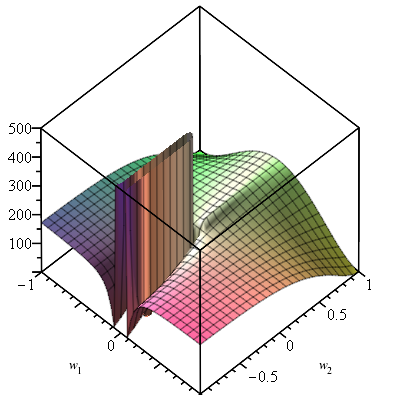
\includegraphics[width=\linewidth,trim={0 0 0 4.35cm},clip]{graphics/nac-mul-eps-1em7.png}
  \caption{$\mathrm{NAC}_{\bullet}$ with $\epsilon = 10^{-7}$}
\end{subfigure}%
\begin{subfigure}{.33\textwidth}
  \centering
  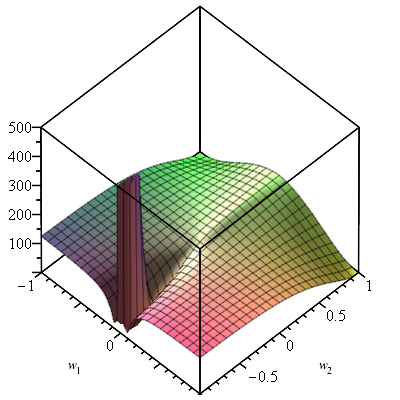
\includegraphics[width=\linewidth,trim={0 0 0 4.35cm},clip]{graphics/nac-mul-eps-1em1.png}
  \caption{$\mathrm{NAC}_{\bullet}$ with $\epsilon = 0.1$}
\end{subfigure}
\begin{subfigure}{.33\textwidth}
  \centering
  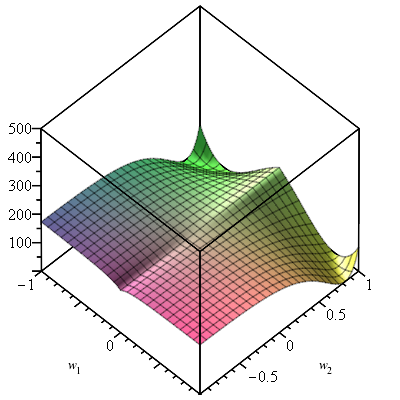
\includegraphics[width=\linewidth,trim={0 0 0 4.35cm},clip]{graphics/nac-mul-eps-1.png}
  \caption{$\epsilon = 1$}
\end{subfigure}
%\begin{subfigure}{.33\textwidth}
%  \centering
%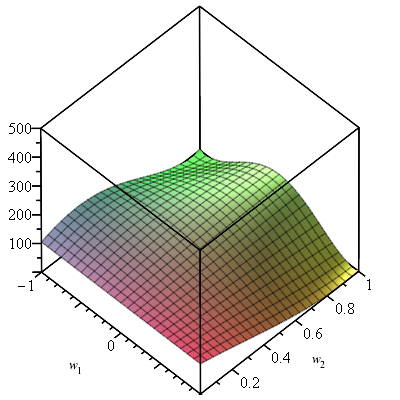
\includegraphics[width=\linewidth]{graphics/nac-mul-nmu.png}
%  \caption{Our NMU solution}
%\end{subfigure}

\caption{RMS loss curvature for a $\mathrm{NAC}_{+}$ layer followed by either a $\mathrm{NAC}_{\bullet}$. The weight matrices constrained are to $\mathbf{W}_1 = \left[\protect\begin{smallmatrix}
w_1 & w_1 & 0 & 0 \\
w_1 & w_1 & w_1 & w_1
\protect\end{smallmatrix}\right]$, $\mathbf{W}_2 = \left[\protect\begin{smallmatrix}
w_2 & w_2
\protect\end{smallmatrix}\right]$. The problem is $(x_1 + x_2) \cdot (x_1 + x_2 + x_3 + x_4)$ for $x = \left(1, 1.2, 1.8, 2\right)$. The desired solution is $w_1 = w_2 = 1$, although this problem have additional undesired unstable solutions.}
\label{fig:nac-mul-eps-issue}
\end{figure}

\subsubsection{Initialization of $\mathrm{NAC}_{\bullet}$}
Initialization is important to consider for fast and consistent convergence, one desired property is that weights can be initialized such that $E[z_{h_\ell}] = 0$ \cite{glorot-initialization}. Using second order Taylor approximation and assuming all $z_{h_{\ell-1}}$ are uncorrelated, the expectation of $\mathrm{NAC}_{\bullet}$ can be estimated as
\begin{equation}
E[z_{h_\ell}] \approx \left(1 + \frac{1}{2} Var[W_{h_\ell, h_{\ell-1}}] \log(|E[z_{h_{\ell-1}}]| + \epsilon)^2\right)^{H_{\ell-1}} \Rightarrow E[z_{h_\ell}] > 1.
\label{eq:nac-mul:expectation}
\end{equation}
As shown in equation \ref{eq:nac-mul:expectation}, satisfying $E[z_{h_\ell}] = 0$ for $\mathrm{NAC}_{\bullet}$ is likely impossible. The variance can also not be input-independent initialized and is expected to explode (proofs in Appendix \ref{sec:appendix:moments:nac-mul}).

\subsubsection{Neural multiplication unit}
To solve the the gradient and initialization challenges for $\mathrm{NAC}_{\bullet}$ we propose a new neural multiplication unit (NMU):

\begin{align}
W_{h_{\ell-1},h_\ell} &= \min(\max(W_{h_{\ell-1},h_\ell}, 0), 1), \\
\mathcal{R}_{\ell,\mathrm{sparse}} &= \frac{1}{H_\ell \cdot H_{\ell-1}} \sum_{h_\ell=1}^{H_\ell} \sum_{h_{\ell-1}=1}^{H_{\ell-1}} \min\left(W_{h_{\ell-1},h_\ell}, 1 - W_{h_{\ell-1},h_\ell}\right) \\
\textrm{NMU}:\ z_{h_\ell} &= \prod_{h_{\ell-1}=1}^{H_{\ell-1}} \left(W_{h_{\ell-1},h_\ell} z_{h_{\ell-1}} + 1 - W_{h_{\ell-1},h_\ell} \right) \label{eq:nmu-defintion}
\end{align}
The NMU is regularized similar to the NAU and has a multiplicative identity when $W_{h_{\ell-1},h_\ell}=0$.
The NMU unit does not support division by design.
%Previous experiments using the NALU for division does not work well on division hence very little is lost with this modification \cite{trask-nalu}.
As opposed to the $\mathrm{NAC}_{\bullet}$, the NMU can represent input of both negative and positive values and is not $\epsilon$ bounded, which allows the NMU to extrapolate to $z_{h_{\ell-1}}$ that are negative or smaller than $\epsilon$. Its gradients are derived in Appendix \ref{sec:appendix:gradient-derivatives:gradient-nmu}.

\subsubsection{Moments and initialization}
Our proposed NAU can be initialized using Glorot initialization as it is a linear layer. The $\mathrm{NAC}_{+}$ unit can also achieve an ideal initialization, although it is less trivial (details in Appendix \ref{sec:appendix:moments:weight-matrix-construction}).

Our proposed NMU is initialized with $E[W_{h_{\ell}, h_{\ell - 1}}] = \nicefrac{1}{2}$. Assuming all $z_{h_{\ell-1}}$ are uncorrelated, and $E[z_{h_{\ell-1}}] = 0$, which is the case for most units, the expectation can be approximated to
\begin{equation}
E[z_{h_\ell}] \approx \left(\frac{1}{2}\right)^{H_{\ell-1}},
\end{equation}
which approaches zero for $H_{\ell-1} \rightarrow \infty$ (see Appendix \ref{sec:appendix:moments:nmu}). The NMU can, assuming $Var[z_{h_{\ell-1}}] = 1$ and $H_{\ell-1}$ is large, be initialized optimally with $Var[W_{h_{\ell-1},h_\ell}] = \frac{1}{4}$ (proof in Appendix \ref{sec:appendix:moments:nmu:initialization}).

\subsubsection{Regularizer scaling}
We use the regularizer scaling as defined in \eqref{eq:regualizer-scaling}. The motivation here, is that the optimization consists of two parts. A warmup period, where $W_{h_{\ell-1},h_\ell}$ should get close to the solution, unhindered by the sparsity regularizer, and then a period where the solution is made sparse.
\begin{equation}
\lambda_{\mathrm{sparse}} = \hat{\lambda}_{\mathrm{sparse}} \max(\min(\frac{t - \lambda_{\mathrm{start}}}{\lambda_{\mathrm{end}} - \lambda_{\mathrm{start}}}, 1), 0)
\label{eq:regualizer-scaling}
\end{equation}
